%-------------------------------
%	PACKAGES AND OTHER DOCUMENT CONFIGURATIONS
%-------------------------------

% The \vref command specifies the location of the reference

%\documentclass[
%10pt, % Main document font size
%a4paper, % Paper type, use 'letterpaper' for US Letter paper
%oneside, % One page layout (no page indentation)
%twoside, % Two page layout (page indentation for binding and different headers)
%headinclude,footinclude, % Extra spacing for the header and footer
%BCOR5mm, % Binding correction
%]{scrartcl}


\documentclass{article}


%--------------------------------------------------------------
%	REQUIRED PACKAGES
%--------------------------------------------------------------

\usepackage[
nochapters, % Turn off chapters since this is an article        
beramono, % Use the Bera Mono font for monospaced text (\texttt)
%eulermath,% Use the Euler font for mathematics
pdfspacing, % Makes use of pdftex’ letter spacing capabilities via the microtype package
dottedtoc % Dotted lines leading to the page numbers in the table of contents
]{classicthesis} % The layout is based on the Classic Thesis style



\usepackage{arsclassica} % Modifies the Classic Thesis package

\usepackage[T1]{fontenc} % Use 8-bit encoding that has 256 glyphs

\usepackage[utf8]{inputenc} % Required for including letters with accents
%--------------------------------------------------------------
% Fonts and languages
\usepackage{libertinus} % The Libertinus font
%\usepackage[adobe-utopia]{mathdesign} % The Utopia font
%\usepackage[p,osf]{scholax}
% T1 and textcomp are loaded by package. Change that here, if you want
% load sans and typewriter packages here, if needed
%\usepackage{amsmath,amsthm}% must be loaded before newtxmath
% amssymb should not be loaded
%\usepackage[scaled=1.075,ncf,vvarbb]{newtxmath}% need to scale up math package
% vvarbb selects the STIX version of blackboard bold.


\usepackage[czech]{babel} % Český jazyk
%--------------------------------------------------------------
\usepackage{graphicx} % Required for including images
\graphicspath{{Figures/}} % Set the default folder for images

\usepackage{enumitem} % Required for manipulating the whitespace between and within lists

\usepackage{lipsum} % Used for inserting dummy 'Lorem ipsum' text into the template

\usepackage{subfig} % Required for creating figures with multiple parts (subfigures)

\usepackage{amsmath,amssymb,amsthm,amsfonts} % For including math equations, theorems, symbols, etc

\usepackage{varioref} % More descriptive referencing

\usepackage[top =3 cm, bottom = 3.5 cm, left = 1.5 cm, right = 1.5 cm]{geometry}

\usepackage{mathtools}

\usepackage{float}

\usepackage{caption}

%------------------------------------------------------------
%	DIAGRAMS AND TIKZ
\usepackage{smartdiagram}
\usepackage{metalogo}
\usepackage{tikz}
\usetikzlibrary{matrix,calc}

\usepackage{hhline} % kvůli double line v tabulkách
%------------------------------------------------------------
%	THEOREM STYLES
%------------------------------------------------------------

\theoremstyle{definition} % Define theorem styles here based on the definition style (used for definitions and examples)
\newtheorem{definition}{Definice}
\newtheorem{example}{Příklad}
\newtheorem{exercise}{Cvičení}

\theoremstyle{plain} % Define theorem styles here based on the plain style (used for theorems, lemmas, propositions)
\newtheorem{theorem}{Věta}

\theoremstyle{remark} % Define theorem styles here based on the remark style (used for remarks and notes)
\newtheorem{remark}{Poznámka}



%-------------------------------------------------------------
%	HYPERLINKS
%-------------------------------------------------------------

\hypersetup{
%draft, % Uncomment to remove all links (useful for printing in black and white)
colorlinks=true, breaklinks=true, bookmarks=true,bookmarksnumbered,
urlcolor=webbrown, linkcolor=RoyalBlue, citecolor=webgreen, % Link colors
pdftitle={}, % PDF title
pdfauthor={\textcopyright}, % PDF Author
pdfsubject={}, % PDF Subject
pdfkeywords={}, % PDF Keywords
pdfcreator={pdfLaTeX}, % PDF Creator
pdfproducer={LaTeX with hyperref and ClassicThesis} % PDF producer
}

 % Include the structure.tex file which specified the document structure and layout

%----------------------------------------------------
%	MATHEMATICS
%----------------------------------------------------

% Tělesa, obory íntegrity a metrické prostory
\newcommand{\C}{\mathbb{C}}
\newcommand{\R}{\mathbb{R}}
\newcommand{\N}{\mathbb{N}}
\newcommand{\Q}{\mathbb{Q}}
\newcommand{\Z}{\mathbb{Z}}
\renewcommand{\L}[2]{L^{#1} \left( #2 \right)} % Lebesgueovy prostory

\newcommand{\vc}[1]{\boldsymbol{#1}} % vektor
\newcommand{\mat}[1]{\mathbf{#1}} % matice

\newcommand{\norm}[1]{\left \Vert #1 \right \Vert} % norma vektoru
\newcommand{\set}[1]{ \left \lbrace #1 \right \rbrace} % množina
\newcommand{\const}{\mathrm{konst}} % konstanta

\newcommand{\F}{\mathcal{F} } % Fourierova transformace
\newcommand{\La}{\mathcal{L}} % Laplaceova transformace

% Označení funkcí
\newcommand{\Res}[2]{\mathrm{Res}_{#1} \, #2 \,} % residuum
\newcommand{\sgn}{\, \mathrm{sign} \,} % signum
\newcommand{\tg}{\,\mathrm{tg}\,} % možné značení tangens


%Značení derivací a integrálů
\newcommand{\der}[2]{\frac{\mathrm{d}#1}{\mathrm{d}#2}} % obyčejná derivace
\newcommand{\pder}[2]{\frac{\partial #1}{\partial #2}} % parciální derivace
\newcommand{\tder}[3]{\left( \pder{#1}{#2} \right)_{#3 = \const}} % termodynamická derivace
\newcommand{\D}{\mathrm{d} } % integrační znamení
\newcommand{\DD}{\mathrm{D}} % absolutní derivace
\newcommand{\intR}{\int_{-\infty}^{\infty}} % integrál přes reálnou osu



% Značení posloupností, limit a sum
\newcommand{\sequence}[2]{ \left \lbrace #1 \right \rbrace_{#2=1}^\infty} % posloupnost
\newcommand{\sumnorm}[1]{\sum_{#1}^\infty} 
\newcommand{\limplus}[1]{\lim_{#1 \rightarrow + \infty}}
\newcommand{\limminus}[1]{\lim_{#1 \rightarrow - \infty}}


% VŠE záležitosti
\newcommand{\dder}[2]{\frac{\Delta #1}{\Delta #2}}


\newcommand{\arctg}{\mathrm{arctg}\,}
\newcommand{\cotg}{\mathrm{cotg}\,}
\newcommand{\arccotg}{\mathrm{arccotg}\,} % Include the mathematics.tex file which uses some mathematical operators

\hyphenation{Fortran hy-phen-ation} % Specify custom hyphenation points in words with dashes where you would like hyphenation to occur, or alternatively, don't put any dashes in a word to stop hyphenation altogether

%-------------------------------
%	TITLE AND AUTHOR(S)
%-------------------------------

%\title{\normalfont\spacedallcaps{Article Title}} % The article title

%\subtitle{Subtitle} % Uncomment to display a subtitle

\author{\spacedlowsmallcaps{Miroslav Burýšek*}} % The article author(s) - author affiliations need to be specified in the AUTHOR AFFILIATIONS block

\date{\today} % An optional date to appear under the author(s)




%-------------------------------------
%	TESTING
%-------------------------------------
% Load packages for testing
\usepackage{blindtext}
%\usepackage{showframe} % Uncomment to show boxes around the text area, margin, header and footer
%\usepackage[inline]{showlabels}  \showlabels[\small\color{JungleGreen}]{}  % Uncomment to output the content of \label commands to the document where they are used


\begin{document}

%-------------------------------------------
%	HEADERS
%-------------------------------------------

\renewcommand{\sectionmark}[1]{\markright{\spacedlowsmallcaps{#1}}} % The header for all pages (oneside) or for even pages (twoside)
%\renewcommand{\subsectionmark}[1]{\markright{\thesubsection~#1}} % Uncomment when using the twoside option - this modifies the header on odd pages
\lehead{\mbox{\llap{\small\thepage\kern1em\color{halfgray} \vline}\color{halfgray}\hspace{0.5em}\rightmark\hfil}} % The header style

\pagestyle{scrheadings} % Enable the headers specified in this block





%-----------------------------------------
%	TABLE OF CONTENTS & LISTS OF FIGURES AND TABLES
%-----------------------------------------

%\maketitle % Print the title/author/date block

\setcounter{tocdepth}{2} % Set the depth of the table of contents to show sections and subsections only

%\tableofcontents % Print the table of contents

%\listoffigures % Print the list of figures

%\listoftables % Print the list of tables






%--------------------------------------
%	ABSTRACT
%--------------------------------------

%\section*{Abstract} % This section will not appear in the table of contents due to the star (\section*)


%---------------------------------------
%	AUTHOR AFFILIATIONS
%---------------------------------------

\let\thefootnote\relax\footnotetext{\textbf{Verze:} \today }

%--------------------------------------

%\newpage % Start the article content on the second page, remove this if you have a longer abstract that goes onto the second page

%\section{Funkce}

\subsection{Elementární funkce}

Elementární funkce jsou takové, které lze složit konečným počtem operací (sčítání, odčítání, násobení, dělení a skládání) z těchto funkcí: konstanta, obecná mocnina, exponenciála, logaritmus, sinus, kosinus, tangens, kontangens, arkussinus, arkuskosinus, arkustangens a arkuskotangens. 

Jiné funkce než elementární v kurzu prakticky nepotkáme. Je jich ale spousta. Příklady neelementárních funkcí si ukážeme, až budeme vybaveni mocnými nástroji, jako je určitý integrál.

\subsection{Definiční obor}

Definiční obor $D(f)$ (též $D_f$) je množina takových čísel, pro která je funkce $f$ definována.

Při určování definičního oboru elementárních funkcí se v podstatě můžeme řídit jednoduchými zásadami.

\begin{enumerate}
    \item Nesmíme dělit nulou.
    \item Sudé odmocniny jsou definované pouze pro nezáporná čísla.
    \item Logaritmus je definovaný pouze pro kladná čísla.
    \item Speciální pozornost si zaslouží funkce $\tan$, $\cot$, $\arcsin$ a $\arccos$.
\end{enumerate}

Kompletní přehled dává tabulka.

\begin{table}[H]
    \centering
    \begin{tabular}{|c|c|c|}
        \hline
        funkce & definiční obor & obor hodnot \\
        \hline
        $x^k$, $k$ je sudé              & $\R$          & $[0, \infty)$ \\ 
        $x^k$, $k$ je liché             & $\R$          & $\R$ \\ 
        $\sqrt[k]{x}$, $k$ je sudé      & $[0, \infty)$ & $[0, \infty)$ \\
        $\sqrt[k]{x}$, $k$ je liché     & $\R$          & $\R$ \\
        $x^\alpha$, $\alpha \in \R$     & $(0, \infty)$ & $(0, \infty)$ \\
        $e^x$                           & $\R$          & $(0, \infty)$ \\
        $a^x$                           & $\R$          & $(0, \infty)$ \\
        $\log x$                        & $(0, \infty)$ & $\R$ \\
        $\sin x$, $\cos x$              & $\R$          & $[0,1]$ \\
        $\tan x$                        & $\R \setminus \set{\pi/2 + k \pi, k \in \Z}$ & $\R$ \\
        $\cot x$                        & $\R \setminus \set{k \pi, k \in \Z}$  & $\R$ \\
        $\arcsin x$                     & $[-1,1]$      & $[-\frac{\pi}{2}, \frac{\pi}{2}]$ \\
        $\arccos x$                     & $[-1,1]$      & $[0,\pi]$ \\
        $\arctan x$                     & $\R$          & $(-\frac{\pi}{2}, \frac{\pi}{2})$ \\
        $\arccot x$                     & $\R$          & $(0,\pi)$ \\
         \hline
    \end{tabular}
    \caption{Tabulka elementárních funkcí. (Je víceméně potřeba umět ji nazpaměť.)}
    \label{tab:funkce}
\end{table}

\subsection{Růst a pokles funkce}
O funkci řekneme, že je \begin{itemize}
    \item \textbf{rostoucí} na intervalu $I$, jestliže pro všechna $x,y \in I$ splňující $x<y$ platí $f(x) < f(y)$,
    \item \textbf{klesající} na intervalu $I$, jestliže pro všechna $x,y \in I$ splňující $x<y$ platí $f(x) < f(y)$,
    \item \textbf{neklesající} na intervalu $I$, jestliže pro všechna $x,y \in I$ splňující $x<y$ platí $f(x) \leq f(y)$,
    \item \textbf{nerostoucí} na intervalu $I$, jestliže pro všechna $x,y \in I$ splňující $x<y$ platí $f(x) \geq f(y)$,
    \item \textbf{konstantní} na intervalu $I$, jestliže pro všechna $x,y \in I$ splňující $x<y$ platí $f(x) = f(y)$,
    \item \textbf{monotónní} na intervalu $I$, jestliže je na něm neklesající, anebo nerostoucí.
\end{itemize}

\begin{figure}[H]
    \centering
    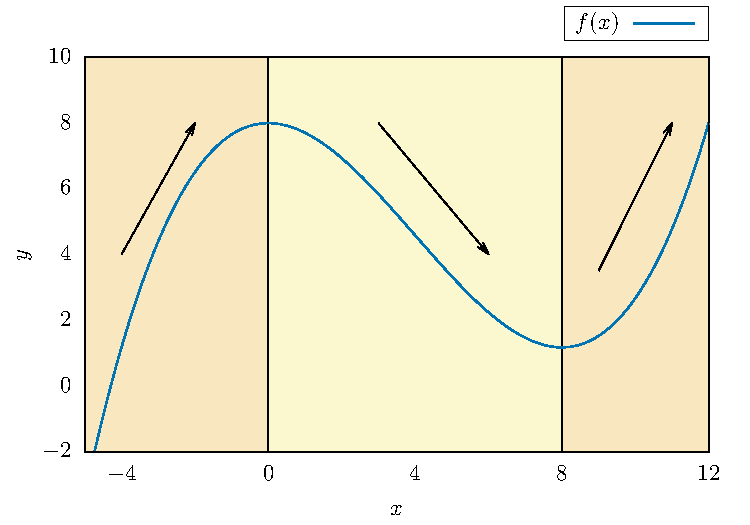
\includegraphics[scale = 0.7]{Gnuplot/Figures/funkce-rostouci-klesajici-obr.pdf}
    \caption{Ilustrace pojmu rostoucí a klesající funkce. Na oranžové oblasti je $f(x)$ rostoucí, na žluté oblasti je $f(x)$ klesající.}
\end{figure}

\begin{remark}
    Pokud mluvíme o růstu nebo poklesu funkce, je vždy nutné uvést, na jakém intervalu se pohybujeme. Důležitost je vidět na následujícím příkladu, viz obrázek \ref{fig:1a-funkce-ne}.

    \begin{figure}[H]
        \centering
        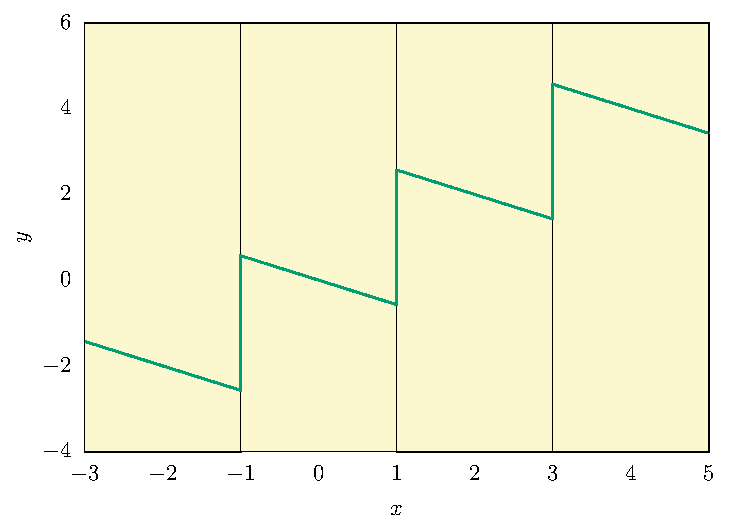
\includegraphics[scale = 0.7]{Gnuplot/Figures/periodicka-klesajici.pdf}
        
        \caption{Příklad funkce, která je klesající na každém intervalu $I_p = (2p-1,2p+1)$, kde $p \in \Z$. Na celém $\R$ ale není ani rostoucí, ani klesající. Porovnáme-li dva body $x_1 < x_2$ v témže intervalu $I_p$, splňují $f(x_1) > f(x_2)$. Porovnáme-li však body v různých intervalech, dostaneme $f(x_1) < f(x_2)$. Není tedy splněna ani jedna z podmínek pro růst nebo pokles na $\R$. Všimněme si, že funkce je v krajních bodech intervalů nespojitá, má v nich skoky.}
        \label{fig:1a-funkce-ne}
    \end{figure}

\end{remark}

\begin{remark}
    V některé literatuře se o různých křivkách mluví jako o \uv{rostoucích zleva doprava} nebo \uv{klesajících zprava doleva} a podobně. Matematická terminologie vždy pracuje s tím, co se děje s hodnotami $f(x)$ \underline{při rostoucích $x$} - tedy vždy \uv{zleva doprava}, chcete-li. Podobně se někdy říká o klesajících funkcích $y(x)$, že \uv{$y$ je nepřímo úměrné $x$}. Ale matematická terminologie říká, že pouze funkce $y(x)=C/x$ je nepřímá úměrnost, žádná jiná funkce toto nesplňuje.

    \begin{figure}[H]
        \centering
        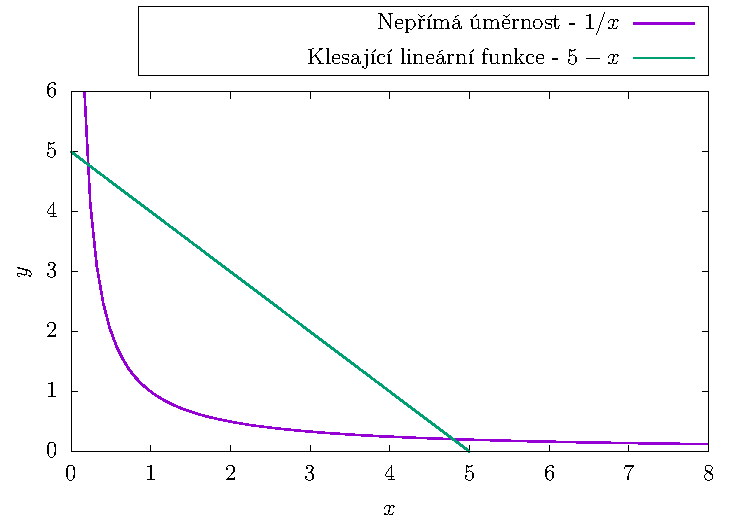
\includegraphics[scale = 0.7]{Gnuplot/Figures/neprima-umernost.pdf}
        \caption{Ilustrace často nesprávně použitého termínu \uv{nepřímá úměrnost}. Pouze funkce typu $C/x$ jsou nepřímé úměrnosti.}
    \end{figure}
\end{remark}

\subsection{Další charakteristiky funkce}

O funkci $f(x)$ říkáme, že je \begin{itemize}
    \item \textbf{prostá} na intervalu $I$, jestliže pro všechna $x,y \in I$ splňující $x \neq y$ platí $f(x) \neq f(y)$ (\uv{každému $x$ přísluší jiná hodnota $f(x)$}),
    \item \textbf{omezená shora}, jestliže existuje konečné číslo $K$ takové, že pro všechna $x \in D(f)$ platí $f(x) \leq K$,
    \item \textbf{omezená zdola}, jestliže existuje konečné číslo $K$ takové, že pro všechna $x \in D(f)$ platí $f(x) \geq K$,
    \item \textbf{omezená}, jestliže je omezená shora i zdola.
\end{itemize}

Jestliže je funkce $f$ prostá na intervalu $I$, pak k ní existuje \textbf{inverzní funkce}, kterou označujeme $f^{-1}$.

\begin{example}
    Funkce $x^2$ je prostá na intervalu $(-\infty, 0]$ a na intervalu $[0,+\infty)$. Není prostá na $\R$, protože $(-2)^2 = 4 = (+2)^2$.

    Na intervalu $[0,\infty)$ k ní existuje inverzní funkce $\sqrt{x}$. Na intervalu $(-\infty,0]$ k ní existuje inverzní funkce $\sqrt{-x}$.
\end{example}



\subsection{Příklady na definiční obor}

\begin{example}
    Určíme definiční obor funkce \begin{align*}
        R(x) = \frac{x^2-1}{(x+1)(x-4)(x^2 + 4x - 5)} \:.
    \end{align*}

    Řešení: První pravidlo nám říká, že nesmíme dělit nulou. Musíme tedy najít všechna $x$ taková, že je jmenovatel zlomku nulový: \begin{align*}
        (x+1)(x-4)(x^2 + 4x - 5) = 0 \:.
    \end{align*}
    Součin čísel (nebo výrazů, závorek) je nulový tehdy a jen tehdy, když je jedno z čísel nulové. Každou závorku tedy řešíme zvlášť:
    \begin{align*}
        \begin{cases}
            x+1 = 0 \Longrightarrow x = -1 \:, \\
        x-4 = 0 \Longrightarrow x = 4 \:, \\
        x^2 + 4x - 5 = 0 \Longrightarrow x = \frac{-4 \pm \sqrt{16+20}}{2} = - 2 \pm 3 \:, \: x = -5, 1
        \end{cases}
         \:.
    \end{align*}
    Tato řešení jsou body, které musíme z definičního oboru vyloučit. Tedy \begin{align*}
        \boxed{D(R) = \R \setminus \set{-5,-1,1,4} }\:.
    \end{align*}
    Poznámka: někdo by snad mohl postupovat tak, že by čitatel rovněž převedl na součin závorek: $x^2-1 = (x-1)(x+1)$. Jmenovatel lze též převést na součin: $x^2+4x-5 = (x+5)(x-1)$. Postupoval by tedy krácením:
    \begin{align*}
        R(x) = \frac{(x-1)(x+1)}{(x+1)(x-4)(x+5)(x-1)} \overset{?}{=} \frac{1}{(x+1)(x-4)} \:.
    \end{align*}
    Výraz na levé straně má jiný definiční obor: $\R \setminus \set{-1,4} \neq D(R)$.
    \textbf{Číselné hodnoty výrazů napravo a nalevo jsou stejné, ale definiční obor výrazů je různý!} Poučení tedy je: nejdříve nalezneme definiční obor a pak můžeme krátit.
\end{example}

\begin{example}
    Ještě jednou upozorníme na stejný případ: funkce $f(x) = \frac{x}{x}$ odpovídá konstantní funkci $g(x) = 1$, s tím rozdílem, že do $f$ nelze dosadit nulu. Takže \begin{align*}
        D(f) = \R \setminus \set{0} \neq \R = D(g) \:.
    \end{align*}
    
\end{example}

\begin{example}
    Určíme definiční obor funkce \begin{align*}
        h(x) = \sqrt{ \frac{\log (x-2)}{x-4}}
    \end{align*}

    Řešení: 1. pravidlo nám vyloučí bod $x=4$. 
    Dále nám 3. pravidlo říká, že do $\log$ můžeme dosadit pouze kladná čísla, takže musí platit $x-2>0$. To odpovídá hodnotám $x \in (2, \infty)$. 
    Konečně nám 2. pravidlo říká, že musí být výraz pod odmocninou nezáporný, musíme tedy řešit nerovnici \begin{align*}
        \frac{\log (x-2)}{x-4} \geq 0 \:.
    \end{align*}
    Nejprve vyřešíme případ, kdy platí rovnost.
    \begin{align*}
        \log (x-2) = 0 \Longrightarrow x-2 = 1 \Longrightarrow x = 3 \:.
    \end{align*}
    
    Nyní vyřešíme případ nerovnosti. Podíl dvou čísel je větší než nula právě tehdy, když jsou obě čísla kladná anebo obě čísla záporná (samozřejmě \uv{minus krát minus je plus}). Stačí tedy řešit podmínky:
    \begin{align*}
        \begin{cases}
            \left [\log (x-2) > 0 \right] \bigwedge \left[ x-4 > 0\right] \Longrightarrow [x \in (3,\infty)] \bigwedge [x \in (4, \infty)] \Longrightarrow x \in (4, \infty) \:, \\
            \left [\log (x-2) < 0 \right] \bigwedge \left[ x-4 < 0\right] \Longrightarrow [x \in (2,3)] \bigwedge [x \in (-\infty, 4)] \Longrightarrow x \in (2,3)
        \end{cases}
         \:.
    \end{align*}
    Celkově máme \begin{align*}
        \boxed{ D(h) = (2,3) \cup \set{3} \cup (4,\infty) = (2,3] \cup (4,\infty) } \:.
    \end{align*}
\end{example}

\begin{example}
    Určíme definiční obor funkce \begin{align*}
        P(x) = \frac{\arcsin (x-1)}{x^x} \:.
    \end{align*}

    Řešení: jmenovatel vyloučí bod nula. Dále, definiční obor funkce $\arcsin$ je $[-1,1]$, tedy $ -1 \leq x-1 \leq 1$, takže $x \in [0,2]$. 
    Nyní se podívejme na funkci ve jmenovateli. Tu můžeme přepsat \begin{align*}
        x^x = \left( e^{\log x} \right) = e^{x \log x} \:,
    \end{align*}
    takže se v ní objeví logaritmus a vidíme, že $x \in (0, \infty)$.
    Celkově \begin{align*}
        \boxed{ D(P) = [0,2] \cap (0, \infty) = (0,2] } \:.
    \end{align*}

\end{example}

\begin{example}
    Určíme definiční obor funkce 
    \begin{align*}
        m(t) = \tan (\sqrt{t+1}) \:.
    \end{align*}

    Řešení: odmocnina dává podmínku $t \in [-1,\infty)$. Dále platí $\tan x = \frac{\sin x}{\cos x} $, takže $\tan (\sqrt {t+1}) = \frac{\sin (\sqrt {t+1})}{\cos (\sqrt {t+1})}$. Protože nesmíme dělit nulou, musíme najít body \begin{align*}
        \cos (\sqrt{t+1}) = 0 \:.
    \end{align*}
    Substitucí $\sqrt{t+1} = u$ dostáváme podmínku $\cos u =0$, která odpovídá bodům $u = \frac{\pi}{2} + k \pi \:, k \in \Z$. Odtud máme \begin{align*}
        \sqrt{t+1} = \frac{\pi}{2} + k \pi \:.
    \end{align*}
    Nyní musíme vyjádřit $t$, což uděláme prostým umocněním a odečtením jedničky:
    \begin{align*}
        t =  \left( \frac{\pi}{2} + k \pi \right)^2 - 1 = \frac{\pi^2}{4} + 2 \cdot k \pi \cdot \frac{\pi}{2} + k^2 \pi^2 - 1 = k^2 \pi^2 + k \pi^2 + \frac{\pi^2}{4} - 1 \:.
    \end{align*}
    Definiční obor je tedy \begin{align*}
        D(m) = \set{t : t \geq -1, t \neq k^2 \pi^2 + k \pi^2 + \frac{\pi^2}{4} - 1, \: k \in \Z} \:.
    \end{align*}
\end{example}

\begin{example}
    Určíme definiční obor funkce \begin{align*}
        g(x) = \frac{\sin^3 x + 4^{-x}}{\sqrt{|2x-1|-|x+1|-3}} \:.
    \end{align*}
    Funkce v čitateli mají definiční obor $\R$. Musíme tedy zařídit, aby odmocnina ve jmenovateli byla dobře definovaná a aby byla nenulová, to znamená zajistit \begin{align*}
        |2x-1|-|x+1|-3 > 0 \:.
    \end{align*}

    Nerovnice s absolutní hodnotou se řeší pomocí tabulek. Nejprve najdeme body, kdy je absolutní hodnota nulová. V našem případě to jsou body $2x-1 = 0 \Rightarrow x=1/2$ a $x+1=0 \Rightarrow x=-1$. Nyní stačí využít toho, že $|x| = +x$ pro $x>0$ a $|x| = -x$ pro $x<0$.

    \begin{table}[H]
        \centering
        \begin{tabular}{c||c|c|c}
            
            \textbf{interval} & $(-\infty,-1)$ & $(-1,1/2)$ & $(1/2, +\infty)$ \\
            \hhline{=#=|=|=} 
            $|2x-1|$ & $-2x+1$ & $-2x+1$ & $+2x-1$ \\
            \hline
            $|x+1|$ & $-x-1$ & $+x+1$ & $+x+1$ \\
            \hhline{=#=|=|=}
            $|2x-1|-|x+1|-3$ & $(-2x+1)-(-x-1)-3$ & $(-2x+1)-(+x+1)-3$ & $(+2x-1)-(+x+1)-3$ \\
            \hline
            po úpravě & $-x-1$ & $ -3x - 3$ & $x-5$
            
        \end{tabular}
    \end{table}
    Nyní musíme vyřešit tři nerovnice \begin{align*}
        -x-1>0 \:, \quad -3x -3 >0 \:, \quad x-5 > 0 
    \end{align*}
    a podívat se, jestli spadají do zadaného intervalu.

    První rovnice odpovídá $x \in (-\infty,-1)$, což je v souladu s intervalem.
    Druhá rovnice odpovídá $x \in (-\infty,-1)$, který už není v souladu s intervalem.
    Třetí rovnice odpovídá $x \in (5, \infty)$, což je v souladu s intervalem.

    Celkově dostáváme 
    \begin{align*}
        \boxed{ D(g) = (-\infty, -1) \cup (5, \infty) } \:.
    \end{align*}
\end{example}

\section*{Goniometrické a cyklometrické funkce}

\textbf{Goniometrické} (též trigonometrické) funkce jsou $\sin x$, $\cos x$, $\tg x$ a $\cotg x$. Funkce k nim inverzní, $\arcsin x$, $\arccos x$, $\arctg x$ a $\arccotg x$ nazýváme \textbf{cyklometrické}.

\subsubsection*{Arkussinus}

Graf funkce $\sin x$ je na obrázku \ref{fig:sinus}. Platí $D(\sin x) = \R$ a $H(\sin x) = [-1,1]$. Nyní potřebujeme vybrat interval, na kterém je tato funkce prostá, abychom k ní mohli nalézt inverzní. Zároveň chceme pokrýt \uv{co největší obor hodnot}. Nabízí se interval $[-\pi/2, \pi/2]$. Definujeme tedy funkci \textbf{arkussinus} $\arcsin x$ předpisem \begin{align}
    D(\arcsin x) = H(\sin x) = [-1,1] \:, \quad H(\arcsin x) = [-\pi/2, \pi/2] \:, \quad \arcsin(x) = y \Longleftrightarrow x = \sin y \:.
\end{align}

\begin{figure}[H]
    \centering
    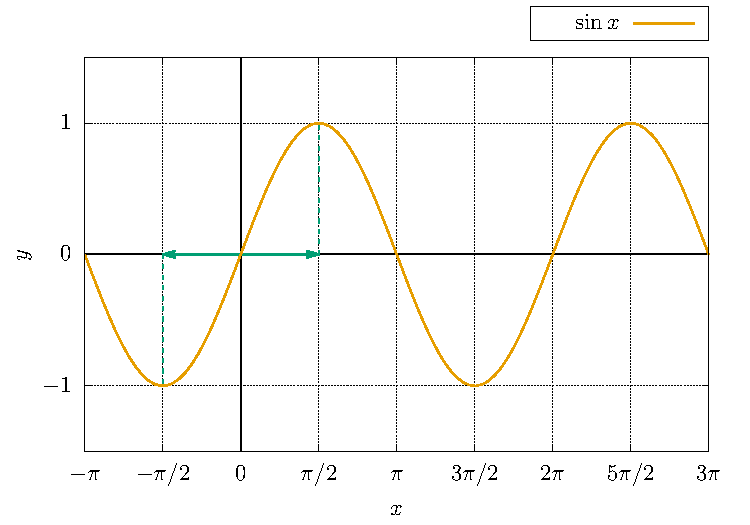
\includegraphics{Gnuplot/cv1/Figures/sinusgraf.pdf}
    \caption{Graf funkce sinus. Zeleně je vyznačen interval, kde je funkce prostá. Ten zvolíme jako obor hodnot funkce arkussinus.}
    \label{fig:sinus}
\end{figure}


\subsubsection*{Arkuskosinus}

Graf funkce $\cos x$ je na obrázku \ref{fig:kosinus}. Platí $D(\cos x) = \R$ a $H(\cos x) = [-1,1]$. Opět se chceme omezit na interval, kde je funkce prostá. Správný interval bude $[0,\pi]$. Definujeme funkci \textbf{arkuskosinus} $\arccos x$ předpisem \begin{align}
    D(\arccos x) = H(\cos x) = [-1,1] \:, \quad H(\arccos x) = [0, \pi] \:, \quad \arccos(x) = y \Longleftrightarrow x = \cos y \:.
\end{align}

\begin{figure}[H]
    \centering
    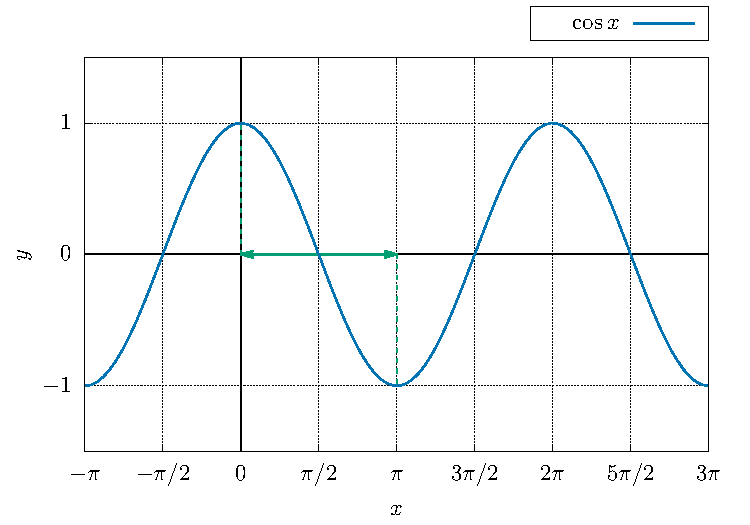
\includegraphics{Gnuplot/cv1/Figures/cosinusgraf.pdf}
    \caption{Graf funkce kosinus. Zeleně je vyznačen interval, kde je funkce prostá. Ten zvolíme jako obor hodnot funkce arkuskosinus.}
    \label{fig:kosinus}
\end{figure}

\subsubsection*{Arkustangens}

Graf funkce $\tg x$ je na obrázku \ref{fig:tangens}. Platí $D(\tg x) = \R \setminus \set{\frac{\pi}{2}+ k \pi, k \in \mathbb{Z}}$ a $H(\tg x) = \R$. Interval, na kterém je funkce prostá, je $(-\pi/2, \pi/2)$. Definujeme funkci \textbf{arkustangens} $\arccos x$ předpisem \begin{align}
    D(\arctg x) = H(\tg x) = \R \:, \quad H(\arctg x) = (-\pi/2, \pi/2) \:, \quad \arctan(x) = y \Longleftrightarrow x = \tg y \:.
\end{align}

\begin{figure}[H]
    \centering
    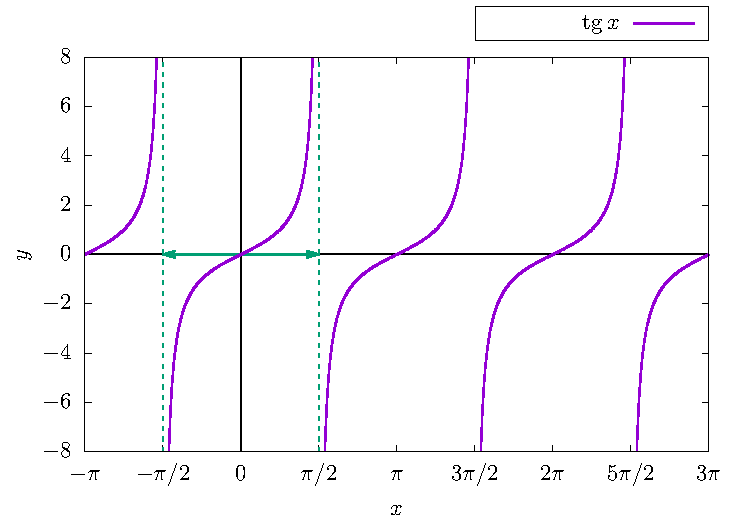
\includegraphics{Gnuplot/cv1/Figures/tangensgraf.pdf}
    \caption{Graf funkce tangens. Zeleně je vyznačen interval, kde je funkce prostá. Ten zvolíme jako obor hodnot funkce arkustangens. Povšimněme si, že v bodech $-\frac{\pi}{2}$ a $\frac{\pi}{2}$ jsou svislé asymptoty. Z nich se stanou vodorovné asymptoty funkce arkustangens.}
    \label{fig:tangens}
\end{figure}

\subsubsection*{Arkuskotangens}

Graf funkce $\cotg x$ je na obrázku \ref{fig:kotangens}. Platí $D(\cotg x) = \R \setminus \set{ k \pi, k \in \mathbb{Z}}$ a $H(\cotg x) = \R$. Interval, na kterém je funkce prostá, je $(0, \pi)$. Definujeme funkci \textbf{arkuskotangens} $\arccotg x$ předpisem 
\begin{align}
    D(\arccotg x) = H(\cotg x) = \R \:, \quad H(\arccotg x) = (0, \pi) \:, \quad \arccotg(x) = y \Longleftrightarrow x = \cotg y \:.
\end{align}

\begin{figure}[H]
    \centering
    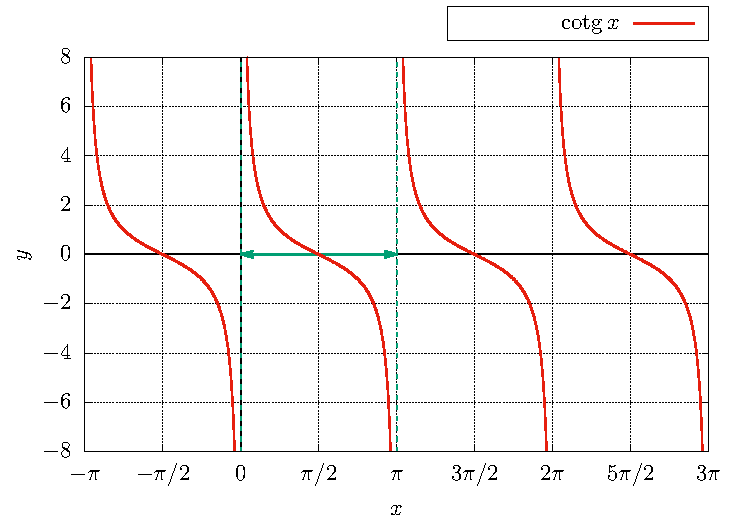
\includegraphics{Gnuplot/cv1/Figures/kotangensgraf.pdf}
    \caption{Graf funkce kotangens. Zeleně je vyznačen interval, kde je funkce prostá. Ten zvolíme jako obor hodnot funkce arkustangens. Povšimněme si, že v bodech $0$ a $\pi$ jsou svislé asymptoty. Z nich se stanou vodorovné asymptoty funkce arkuskotangens.}
    \label{fig:kotangens}
\end{figure}


Grafy funkcí $\arcsin x$ a $\arccos x$ jsou na obrázku \ref{obr:arcsin-arccos}, grafy $\arctg x$ a $\arccotg x$ jsou na obrázku \ref{obr:arctan-arccot}.

\begin{figure}[H]
    \centering
    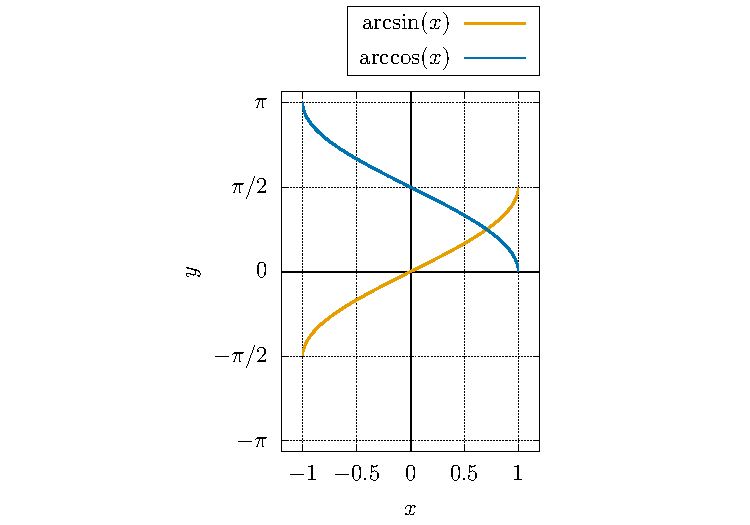
\includegraphics{Gnuplot/cv1/Figures/arcsin-arccos.pdf}
    \caption{Graf funkcí arkussinus a arkuskosinus.}
    \label{obr:arcsin-arccos}
\end{figure}
\begin{figure}[H]
    \centering
    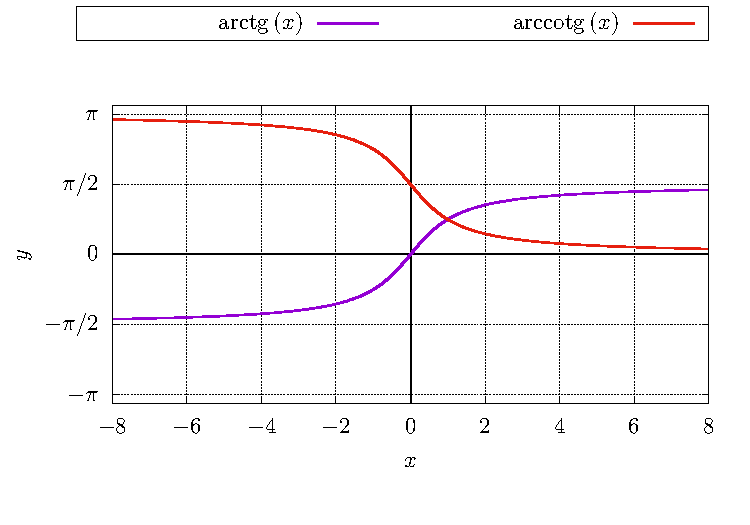
\includegraphics{Gnuplot/cv1/Figures/arctg-arccotg.pdf}
    \caption{Graf funkcí arkustangens a arkuskotangens.}
    \label{obr:arctan-arccot}
\end{figure}

%\subsection{Definiční obor}

Při určování definičního oboru elementárních funkcí se v podstatě můžeme řídit jednoduchými zásadami.

\begin{enumerate}
    \item Nesmíme dělit nulou.
    \item Sudé odmocniny jsou definované pouze pro nezáporná čísla.
    \item Logaritmus je definovaný pouze pro kladná čísla.
    \item Speciální pozornost si zaslouží funkce $\tan$, $\cot$, $\arcsin$ a $\arccos$.
\end{enumerate}

Kompletní přehled dává tabulka \ref{tab:funkce}.

\begin{table}[H]
    \centering
    \begin{tabular}{|c|c|c|}
        \hline
        funkce & definiční obor & obor hodnot \\
        \hline
        $x^k$, $k$ je sudé              & $\R$          & $[0, \infty)$ \\ 
        $x^k$, $k$ je liché             & $\R$          & $\R$ \\ 
        $\sqrt[k]{x}$, $k$ je sudé      & $[0, \infty)$ & $[0, \infty)$ \\
        $\sqrt[k]{x}$, $k$ je liché     & $\R$          & $\R$ \\
        $x^\alpha$, $\alpha \in \R$     & $(0, \infty)$ & $(0, \infty)$ \\
        $e^x$                           & $\R$          & $(0, \infty)$ \\
        $a^x$                           & $\R$          & $(0, \infty)$ \\
        $\log x$                        & $(0, \infty)$ & $\R$ \\
        $\sin x$, $\cos x$              & $\R$          & $[0,1]$ \\
        $\tan x$                        & $\R \setminus \set{\pi/2 + k \pi, k \in \Z}$ & $\R$ \\
        $\cot x$                        & $\R \setminus \set{k \pi, k \in \Z}$  & $\R$ \\
        $\arcsin x$                     & $[-1,1]$      & $[-\frac{\pi}{2}, \frac{\pi}{2}]$ \\
        $\arccos x$                     & $[-1,1]$      & $[0,\pi]$ \\
        $\arctan x$                     & $\R$          & $(-\frac{\pi}{2}, \frac{\pi}{2})$ \\
        $\arccot x$                     & $\R$          & $(0,\pi)$ \\
         \hline
    \end{tabular}
    \caption{Tabulka elementárních funkcí. (Je víceméně potřeba umět ji nazpaměť.)}
    \label{tab:funkce}
\end{table}

\subsection{Příklady na definiční obor}

\begin{example}
    Určíme definiční obor funkce \begin{align*}
        R(x) = \frac{x^2-1}{(x+1)(x-4)(x^2 + 4x - 5)} \:.
    \end{align*}

    Řešení: První pravidlo nám říká, že nesmíme dělit nulou. Musíme tedy najít všechna $x$ taková, že je jmenovatel zlomku nulový: \begin{align*}
        (x+1)(x-4)(x^2 + 4x - 5) = 0 \:.
    \end{align*}
    Součin čísel (nebo výrazů, závorek) je nulový tehdy a jen tehdy, když je jedno z čísel nulové. Každou závorku tedy řešíme zvlášť:
    \begin{align*}
        \begin{cases}
            x+1 = 0 \Longrightarrow x = -1 \:, \\
        x-4 = 0 \Longrightarrow x = 4 \:, \\
        x^2 + 4x - 5 = 0 \Longrightarrow x = \frac{-4 \pm \sqrt{16+20}}{2} = - 2 \pm 3 \:, \: x = -5, 1
        \end{cases}
         \:.
    \end{align*}
    Tato řešení jsou body, které musíme z definičního oboru vyloučit. Tedy \begin{align*}
        \boxed{D(R) = \R \setminus \set{-5,-1,1,4} }\:.
    \end{align*}
    Poznámka: někdo by snad mohl postupovat tak, že by čitatel rovněž převedl na součin závorek: $x^2-1 = (x-1)(x+1)$. Jmenovatel lze též převést na součin: $x^2+4x-5 = (x+5)(x-1)$. Postupoval by tedy krácením:
    \begin{align*}
        R(x) = \frac{(x-1)(x+1)}{(x+1)(x-4)(x+5)(x-1)} \overset{?}{=} \frac{1}{(x+1)(x-4)} \:.
    \end{align*}
    Výraz na levé straně má jiný definiční obor: $\R \setminus \set{-1,4} \neq D(R)$.
    \textbf{Číselné hodnoty výrazů napravo a nalevo jsou stejné, ale definiční obor výrazů je různý!} Poučení tedy je: nejdříve nalezneme definiční obor a pak můžeme krátit.
\end{example}

\begin{example}
    Ještě jednou upozorníme na stejný případ: funkce $f(x) = \frac{x}{x}$ odpovídá konstantní funkci $g(x) = 1$, s tím rozdílem, že do $f$ nelze dosadit nulu. Takže \begin{align*}
        D(f) = \R \setminus \set{0} \neq \R = D(g) \:.
    \end{align*}
    
\end{example}

\begin{example}
    Určíme definiční obor funkce \begin{align*}
        h(x) = \sqrt{ \frac{\log (x-2)}{x-4}}
    \end{align*}

    Řešení: 1. pravidlo nám vyloučí bod $x=4$. 
    Dále nám 3. pravidlo říká, že do $\log$ můžeme dosadit pouze kladná čísla, takže musí platit $x-2>0$. To odpovídá hodnotám $x \in (2, \infty)$. 
    Konečně nám 2. pravidlo říká, že musí být výraz pod odmocninou nezáporný, musíme tedy řešit nerovnici \begin{align*}
        \frac{\log (x-2)}{x-4} \geq 0 \:.
    \end{align*}
    Nejprve vyřešíme případ, kdy platí rovnost.
    \begin{align*}
        \log (x-2) = 0 \Longrightarrow x-2 = 1 \Longrightarrow x = 3 \:.
    \end{align*}
    
    Nyní vyřešíme případ nerovnosti. Podíl dvou čísel je větší než nula právě tehdy, když jsou obě čísla kladná anebo obě čísla záporná (samozřejmě \uv{minus krát minus je plus}). Stačí tedy řešit podmínky:
    \begin{align*}
        \begin{cases}
            \left [\log (x-2) > 0 \right] \bigwedge \left[ x-4 > 0\right] \Longrightarrow [x \in (3,\infty)] \bigwedge [x \in (4, \infty)] \Longrightarrow x \in (4, \infty) \:, \\
            \left [\log (x-2) < 0 \right] \bigwedge \left[ x-4 < 0\right] \Longrightarrow [x \in (2,3)] \bigwedge [x \in (-\infty, 4)] \Longrightarrow x \in (2,3)
        \end{cases}
         \:.
    \end{align*}
    Celkově máme \begin{align*}
        \boxed{ D(h) = (2,3) \cup \set{3} \cup (4,\infty) = (2,3] \cup (4,\infty) } \:.
    \end{align*}
\end{example}

\begin{example}
    Určíme definiční obor funkce \begin{align*}
        P(x) = \frac{\arcsin (x-1)}{x^x} \:.
    \end{align*}

    Řešení: jmenovatel vyloučí bod nula. Dále, definiční obor funkce $\arcsin$ je $[-1,1]$, tedy $ -1 \leq x-1 \leq 1$, takže $x \in [0,2]$. 
    Nyní se podívejme na funkci ve jmenovateli. Tu můžeme přepsat \begin{align*}
        x^x = \left( e^{\log x} \right) = e^{x \log x} \:,
    \end{align*}
    takže se v ní objeví logaritmus a vidíme, že $x \in (0, \infty)$.
    Celkově \begin{align*}
        \boxed{ D(P) = [0,2] \cap (0, \infty) = (0,2] } \:.
    \end{align*}

\end{example}

\begin{example}
    Určíme definiční obor funkce 
    \begin{align*}
        m(t) = \tan (\sqrt{t+1}) \:.
    \end{align*}

    Řešení: odmocnina dává podmínku $t \in [-1,\infty)$. Dále platí $\tan x = \frac{\sin x}{\cos x} $, takže $\tan (\sqrt {t+1}) = \frac{\sin (\sqrt {t+1})}{\cos (\sqrt {t+1})}$. Protože nesmíme dělit nulou, musíme najít body \begin{align*}
        \cos (\sqrt{t+1}) = 0 \:.
    \end{align*}
    Substitucí $\sqrt{t+1} = u$ dostáváme podmínku $\cos u =0$, která odpovídá bodům $u = \frac{\pi}{2} + k \pi \:, k \in \Z$. Odtud máme \begin{align*}
        \sqrt{t+1} = \frac{\pi}{2} + k \pi \:.
    \end{align*}
    Nyní musíme vyjádřit $t$, což uděláme prostým umocněním a odečtením jedničky:
    \begin{align*}
        t =  \left( \frac{\pi}{2} + k \pi \right)^2 - 1 = \frac{\pi^2}{4} + 2 \cdot k \pi \cdot \frac{\pi}{2} + k^2 \pi^2 - 1 = k^2 \pi^2 + k \pi^2 + \frac{\pi^2}{4} - 1 \:.
    \end{align*}
    Definiční obor je tedy \begin{align*}
        D(m) = \set{t : t \geq -1, t \neq k^2 \pi^2 + k \pi^2 + \frac{\pi^2}{4} - 1, \: k \in \Z} \:.
    \end{align*}
\end{example}

\begin{example}
    Určíme definiční obor funkce \begin{align*}
        g(x) = \frac{\sin^3 x + 4^{-x}}{\sqrt{|2x-1|-|x+1|-3}} \:.
    \end{align*}
    Funkce v čitateli mají definiční obor $\R$. Musíme tedy zařídit, aby odmocnina ve jmenovateli byla dobře definovaná a aby byla nenulová, to znamená zajistit \begin{align*}
        |2x-1|-|x+1|-3 > 0 \:.
    \end{align*}

    Nerovnice s absolutní hodnotou se řeší pomocí tabulek. Nejprve najdeme body, kdy je absolutní hodnota nulová. V našem případě to jsou body $2x-1 = 0 \Rightarrow x=1/2$ a $x+1=0 \Rightarrow x=-1$. Nyní stačí využít toho, že $|x| = +x$ pro $x>0$ a $|x| = -x$ pro $x<0$.

    \begin{table}[H]
        \centering
        \begin{tabular}{c||c|c|c}
            
            \textbf{interval} & $(-\infty,-1)$ & $(-1,1/2)$ & $(1/2, +\infty)$ \\
            \hhline{=#=|=|=} 
            $|2x-1|$ & $-2x+1$ & $-2x+1$ & $+2x-1$ \\
            \hline
            $|x+1|$ & $-x-1$ & $+x+1$ & $+x+1$ \\
            \hhline{=#=|=|=}
            $|2x-1|-|x+1|-3$ & $(-2x+1)-(-x-1)-3$ & $(-2x+1)-(+x+1)-3$ & $(+2x-1)-(+x+1)-3$ \\
            \hline
            po úpravě & $-x-1$ & $ -3x - 3$ & $x-5$
            
        \end{tabular}
    \end{table}
    Nyní musíme vyřešit tři nerovnice \begin{align*}
        -x-1>0 \:, \quad -3x -3 >0 \:, \quad x-5 > 0 
    \end{align*}
    a podívat se, jestli spadají do zadaného intervalu.

    První rovnice odpovídá $x \in (-\infty,-1)$, což je v souladu s intervalem.
    Druhá rovnice odpovídá $x \in (-\infty,-1)$, který už není v souladu s intervalem.
    Třetí rovnice odpovídá $x \in (5, \infty)$, což je v souladu s intervalem.

    Celkově dostáváme 
    \begin{align*}
        \boxed{ D(g) = (-\infty, -1) \cup (5, \infty) } \:.
    \end{align*}
\end{example}

%%-------------------------------------
%	BIBLIOGRAPHY
%-------------------------------------

\renewcommand{\refname}{\spacedlowsmallcaps{References}} % For modifying the bibliography heading

\bibliographystyle{unsrt}

\bibliography{sample.bib} % The file containing the bibliography

%------------------------------------

\end{document}